\documentclass[10pt,a4paper]{article}
\usepackage[T1]{fontenc}
\usepackage{lmodern}
\usepackage{microtype}
\usepackage[margin=1.6cm,top=1.3cm,bottom=1.2cm]{geometry}
\usepackage{graphicx}
\usepackage{enumitem}
\usepackage[colorlinks=true,urlcolor=blue]{hyperref}
\pagestyle{empty}
\setlist{itemsep=1.5pt,topsep=2pt,leftmargin=14pt}
\setlength{\parindent}{0pt}
\setlength{\parskip}{4pt}
\setlength{\emergencystretch}{2em}
\newcommand{\head}[1]{\vspace{2pt}{\large\bfseries #1}\par\vspace{1pt}}

\begin{document}

{\LARGE\bfseries Time-Series Momentum in a Ten-ETF Universe}\par
\vspace{2pt}
{\large Volatility targeting, regime overlay and crisis performance, 2008 to 2026: one-page summary}\par
\vspace{2pt}
Zack Higham, BSc Mathematics, Queen Mary University of London. Full paper (27 pages) and code:\par
{\small\href{https://github.com/zack-higham/Time-Series-Momentum-with-Volatility-Targeting-and-Regime-Conditioned-Exposure}{github.com/zack-higham/Time-Series-Momentum-with-Volatility-Targeting-and-Regime-Conditioned-Exposure}}

\head{Question}
Does a multi-asset time-series momentum (TSMOM) strategy built only from liquid ETFs earn a positive risk-adjusted return, which layer of the strategy drives it, does it pay off when equities fall, and is it worth holding beside a conventional portfolio?

\head{Data and design}
Ten ETFs in four asset classes (equities SPY, EFA, EEM; Treasuries IEF, TLT; commodities GLD, DBC; currencies UUP, FXY, FXA), daily total returns in excess of T-bills, 222 months from April 2008 to September 2026, 10 bps per unit traded. Every parameter was committed to git before the first backtest.
\begin{itemize}
\item \textbf{Signal (V1):} long or short each ETF by the sign of its trailing 12-month excess return.
\item \textbf{Volatility targeting (V2, primary):} equal ex-ante risk per asset class, scaled to 10\% portfolio volatility.
\item \textbf{Regime overlay (V3):} exposure scaled by a walk-forward Markov-switching model's filtered probability that trend is paying.
\end{itemize}

\head{Findings}
\begin{enumerate}
\item \textbf{Volatility targeting is the layer that matters.} V2: Sharpe 0.45 (V1: 0.26), maximum drawdown $-26.8\%$, monthly skew turned from $-0.50$ to $+0.33$; the gain over V1 is not significant (bootstrap $p = 0.19$). Correlation 0.77 with the AQR futures TSMOM factor validates the ETF implementation.
\item \textbf{Crisis performance.} V2 gained 9.2\%, 12.6\% and 30.6\% in the three largest equity drawdowns (2008 to 2009, 2020, 2022) while SPY fell 51.8\%, 33.8\% and 25.3\%.
\item \textbf{As a diversifier (pre-specified 80/20 blend).} Adding 20\% V2 to a 60/40 portfolio cut its maximum drawdown from $-32.3\%$ to $-25.3\%$ and its loss in all six equity crisis windows (2022: $-21.6\%$ to $-12.6\%$), at a lower mean. Sharpe rose from 0.74 to 0.86, not significant ($p = 0.08$).
\item \textbf{Regime timing fails out of sample.} The walk-forward overlay lowers the Sharpe ratio to 0.39; the same overlay with full-sample smoothed probabilities would have shown a spurious 0.57, an illustration of lookahead bias.
\item \textbf{Honest significance.} Deflated for the 25 configurations examined, V2's Sharpe ratio is not significant (DSR 0.68).
\end{enumerate}

\begin{center}
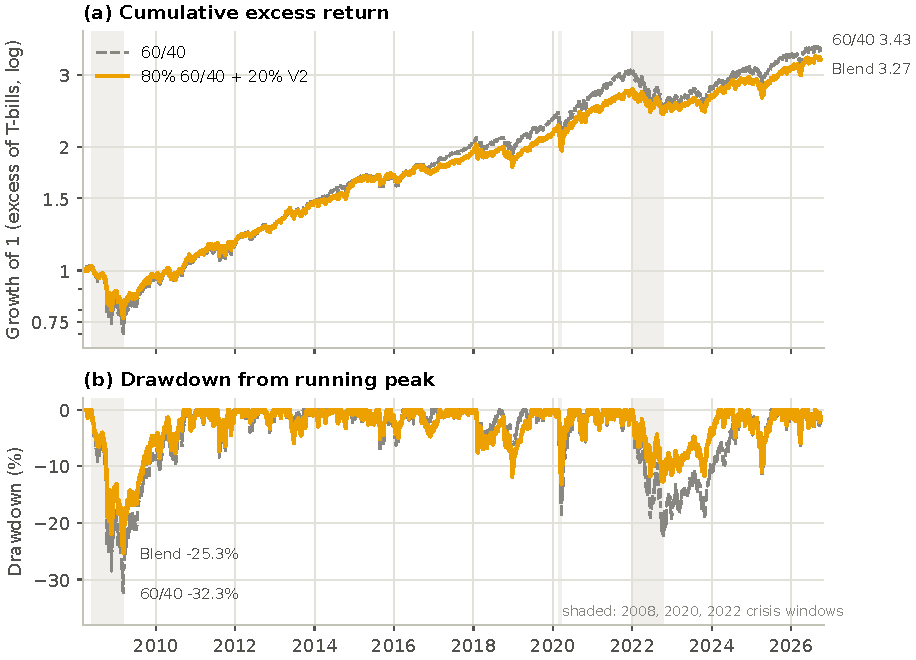
\includegraphics[height=6.1cm]{figures/fig10_blend.pdf}\\[-1pt]
{\small 60/40 against 80\% 60/40 + 20\% V2: growth in excess of T-bills and drawdowns (shaded: crisis windows).}
\end{center}

\head{Main limitation}
One 18.5-year sample with one long bond rally and one sharp rate rise, the episodes behind both V2's crisis gains and the blend's lower drawdowns; ten ETFs give low breadth, and a Sharpe standard error of about 0.23 means no comparison between variants is statistically significant. The ETF implementation also needs leverage (gross 2.15) and shorting, whose costs can remove a quarter of the Sharpe ratio.

\end{document}
